
\documentclass[border=3pt,tikz]{standalone}
\tikzset{
  pics/earth/.style={ % Earth in orbit (argument #1 = polar angle)
    code={
      \message{^^JEarth polar angle=#1}
      \coordinate (-O) at (#1:{\ROx} and {\ROy});
      \begin{scope}[shift={(-O)}]
        \fill[blue!50!cyan!50] (0,0) circle(\RE); % Earth fill (even)
        \fill[blue!20!black!50,rotate=0,opacity=0.9] % Earth shadow
          \ifnum #1=0 (90:\RE) arc(90:-90:\RE) \fi % right shadow
          \ifnum #1=180 (90:\RE) arc(90:270:\RE) \fi % left shadow
          \ifnum #1=270 (0,0) circle(\RE) \fi; % full shadow
        \draw[black,very thin] (0,0) circle(\RE); % Earth outline
      \end{scope}
    }
  }
}
\begin{document}
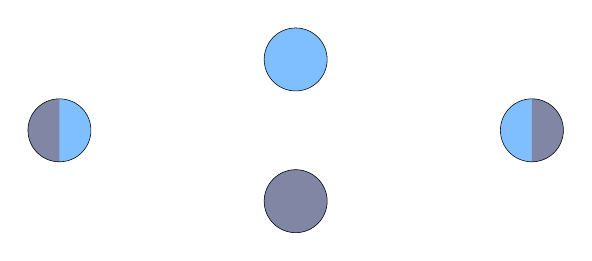
\begin{tikzpicture}
  \def\angE{23} % Earth axis tilt
  \def\RE{0.4} % Earth radius
  \def\ROx{3.0} % orbit horizontal radius
  \def\ROy{0.9} % orbit vertical radius
  \foreach \ang in {0,90,180,270}{
    \pic {earth=\ang};
  }
\end{tikzpicture}
\end{document}
